\documentclass{standalone}

\usepackage{tikz}
\usetikzlibrary{automata, positioning}

\begin{document}
    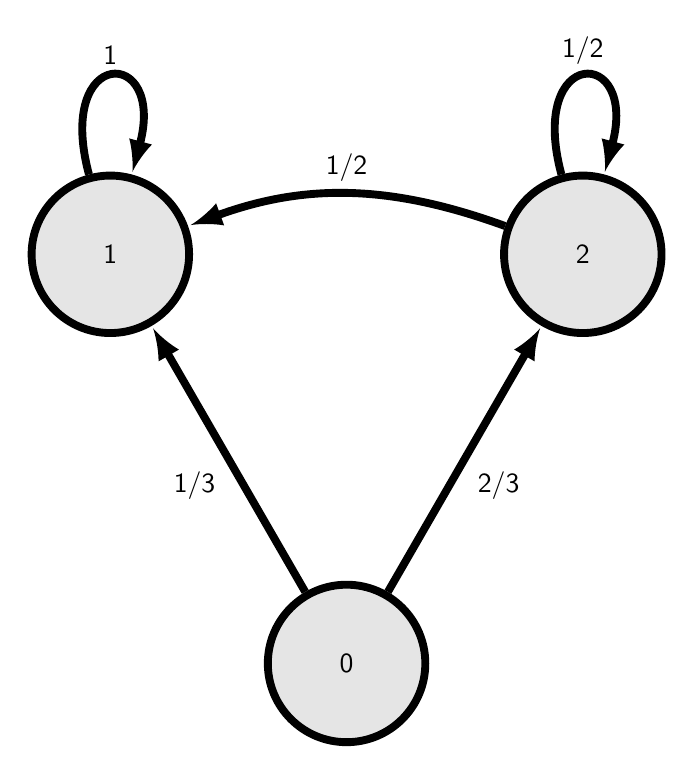
\begin{tikzpicture}[font=\sffamily]

        % Setup the style for the states
        \tikzset{node style/.style={state,
                                    minimum width=2cm,
                                    line width=1mm,
                                    fill=gray!20!white}}

        % Draw the states
				\node[node style] at (3, -5.196) (A) {0};
				\node[node style] at (0, 0)     (B)     {1};
        \node[node style] at (6, 0)     (C)     {2};


        % Connect the states with arrows
        \draw[every loop,
              auto=right,
              line width=1mm,
              >=latex,
              draw=black,
              fill=black]
            (A)     edge           node [swap] {1/3} (B)
						(A)			edge					node {2/3} (C)
						(C) 		edge[loop above]					node {1/2} (C)
						(B) 		edge[loop above]					node {1} (B)
            (C) edge[bend right=20, auto=left] node [swap] {1/2} (B);
    \end{tikzpicture}
\end{document}
